\documentclass[13pt, a4paper, twoside]{article}
\usepackage[utf8]{inputenc}
\usepackage{geometry}
\usepackage[czech]{babel}
\usepackage{enumitem}
\usepackage{fancyhdr}
\usepackage{amsmath}
\usepackage{mathtools}
\usepackage{float}
\usepackage{setspace}
\usepackage{multicol}
\usepackage{graphicx}
\geometry{legalpaper, margin=1.05in}
\pagestyle{fancy}
\lhead{\Large Discussion based assessment}
\rhead{\large Matěj Červenka 2.3.2022}
\begin{document}
\begin{enumerate}
\large \onehalfspacing
\item \textbf{A} 
\begin{figure}[H]
    \centering
    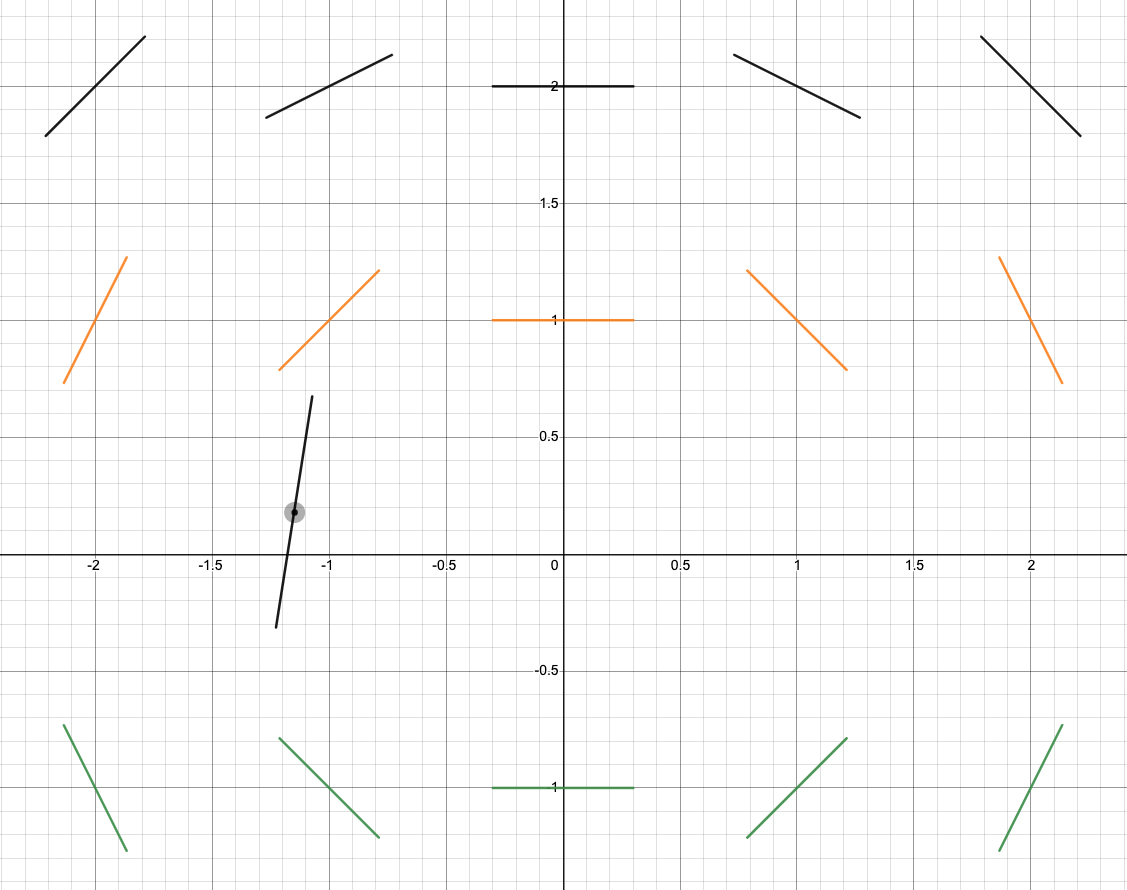
\includegraphics[width=4in]{slope_field.png}
\end{figure}
\textbf{B} The slopes will be negative in I. and III. quadrants
because $\frac{dy}{dx}< 0$ for those xy values. 


\textbf{C} To find the line tangent to $f(1)$ first we need to solve for
$f'(1)$.
\begin{align*}
    f'(1) = \frac{dy}{dx}|_{x=1; y=-1} = 1
\end{align*} 
Now we find the slope equation.
\begin{align*}
    y-1 = 1(x-1)\\ 
    L(x) = x-2
\end{align*}
Now we find the approximation for $f(1.2)$
\begin{align*}
    L(1.2) = 1.2-2 = -0.8
\end{align*}


\textbf{D} First we need to findthe general equation of the differential
equation.
\begin{align*}
    \frac{dy}{dx} &=-\frac{x}{y}\\ 
    \int y dy &= \int -x dx \\
    y^2 &= -x^2 + C \\ 
    y &= \pm \sqrt{-x^2 + C} 
\end{align*}
Now we'll find $C$
\begin{align*}
    1 &= -\sqrt{-1 + C} \\
    C &= 2 \Rightarrow \: \text{There's not a solution for } +\sqrt{-x^2+C}
\end{align*}
Our solution with the given initial condition is $y = -\sqrt{-x^2 + 2}$

\item \textbf{A} To estimate amount of product after a quarter of a year.
We need to find the $A'(0)$
\begin{align*}
    A'(0) = \frac{dA}{dt}|_{t=0; A=1100} = 100
\end{align*}
\newpage
Now we'll use the point-slope formula to find the tangent line and 
then substitute for $t=1/4$.
\begin{align*}
    A - 1100 &= 100t\\
    A &= 100t + 1100 \\ 
    L(\frac{1}{4}) &= 100\cdot \frac{1}{4} + 1100 = 1125 \: tons
\end{align*}

\textbf{B} Solve for $\frac{d^2y}{dt^2}$.
\begin{align*}
    \frac{d^2y}{dt^2} = \frac{d}{dt}(\frac{A}{10}-10) = \frac{1}{10}\frac{dA}{dt} = \frac{1}{100}(A-10)
\end{align*}
We can see that the second derivative will be greater than zero at 
$t=1/4$. So the graph will be concave up there. That means that our 
approximation is an underestimation.

\textbf{C} We'll solve the differential equation with initial condition
$A(0)=1100$.

\begin{align*}
    \frac{dA}{dt}&=\frac{1}{10}(A-100)\\
    \int (A-100)dA &= \int \frac{1}{10}dt\\ 
    ln|A-100| &= \frac{t}{10} + C \\ 
    A - 100 &= Ce^{\frac{t}{10}} \\ 
    A &= 1100e^{\frac{t}{10}} + 100 \Rightarrow \: \text{Because } C=A(0)
\end{align*}

\end{enumerate}
\end{document}